\chapter{Конструкторский раздел}
\label{cha:design}

\section{Модель}
\begin{figure}
    \centering
    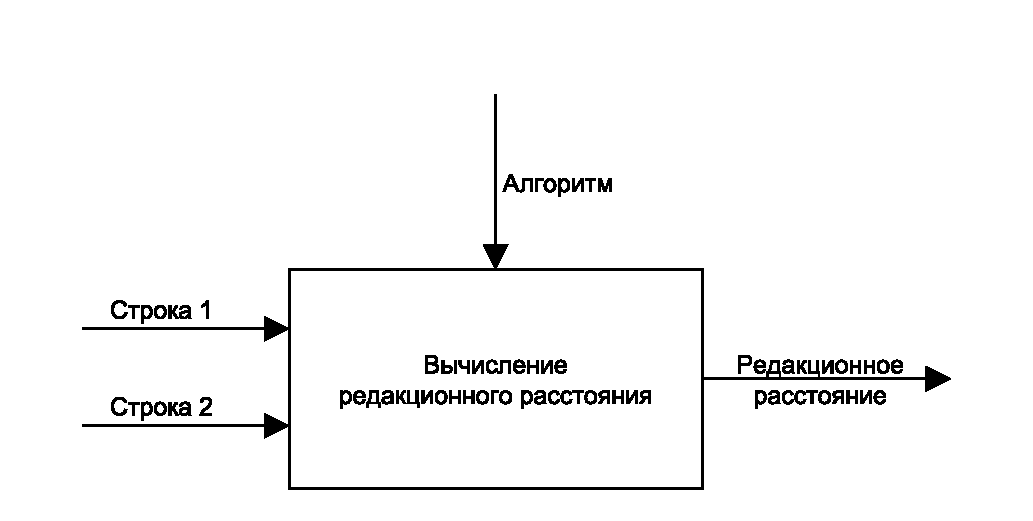
\includegraphics{pdf/mainIdef0.pdf}
    \caption{IDEF\O{} модель}
\end{figure}

\section{Разработка алгоритмов}
Для непосредственной реализации вышеописанных алгоритмов важно иметь их некоторые упрощённые формальные представления, так как чтение таких представлений упрощает написание кода. Подходящим для этого вариантом визуализации являются схемы алгоритмов.

\subsection{Алгоритм Вагнера-Фишера}
Алгоритм Вагнера-Фишера является матричной реализацией поиска расстояния Левенштейна. Ниже приведена схема данного алгоритма.
\begin{figure}[H]
    \centering
    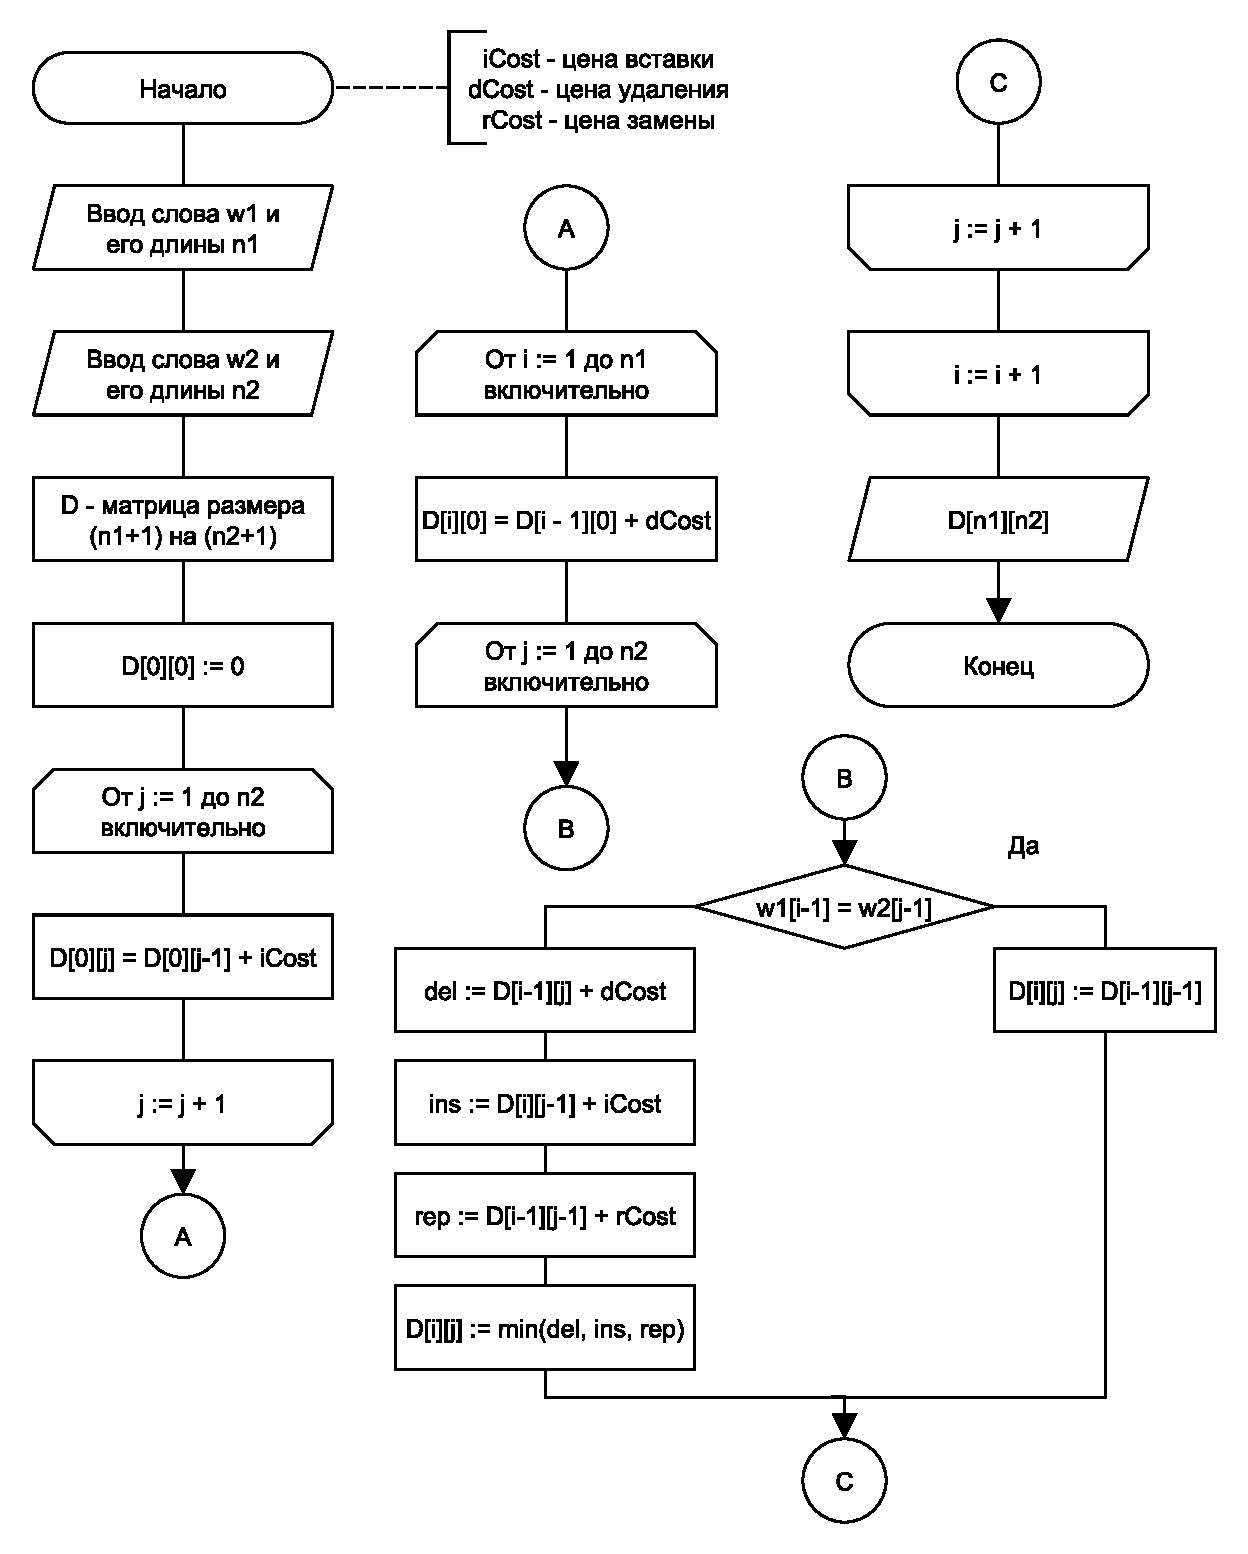
\includegraphics[scale=0.8]{pdf/wagner-fischer-all.pdf}
    \caption{Алгоритм Вагнера-Фишера}
\end{figure}

\subsection{Матричный алгоритм Дамерау-Левенштейна}
Матричный алгоритм Дамерау-Левенштейна представляет из себя модификацию алгоритма Вагнера-Фишера, в которой происходит дополнительная проверка на возможность проведения операции транспозиции.
\begin{figure}[H]
    \centering
    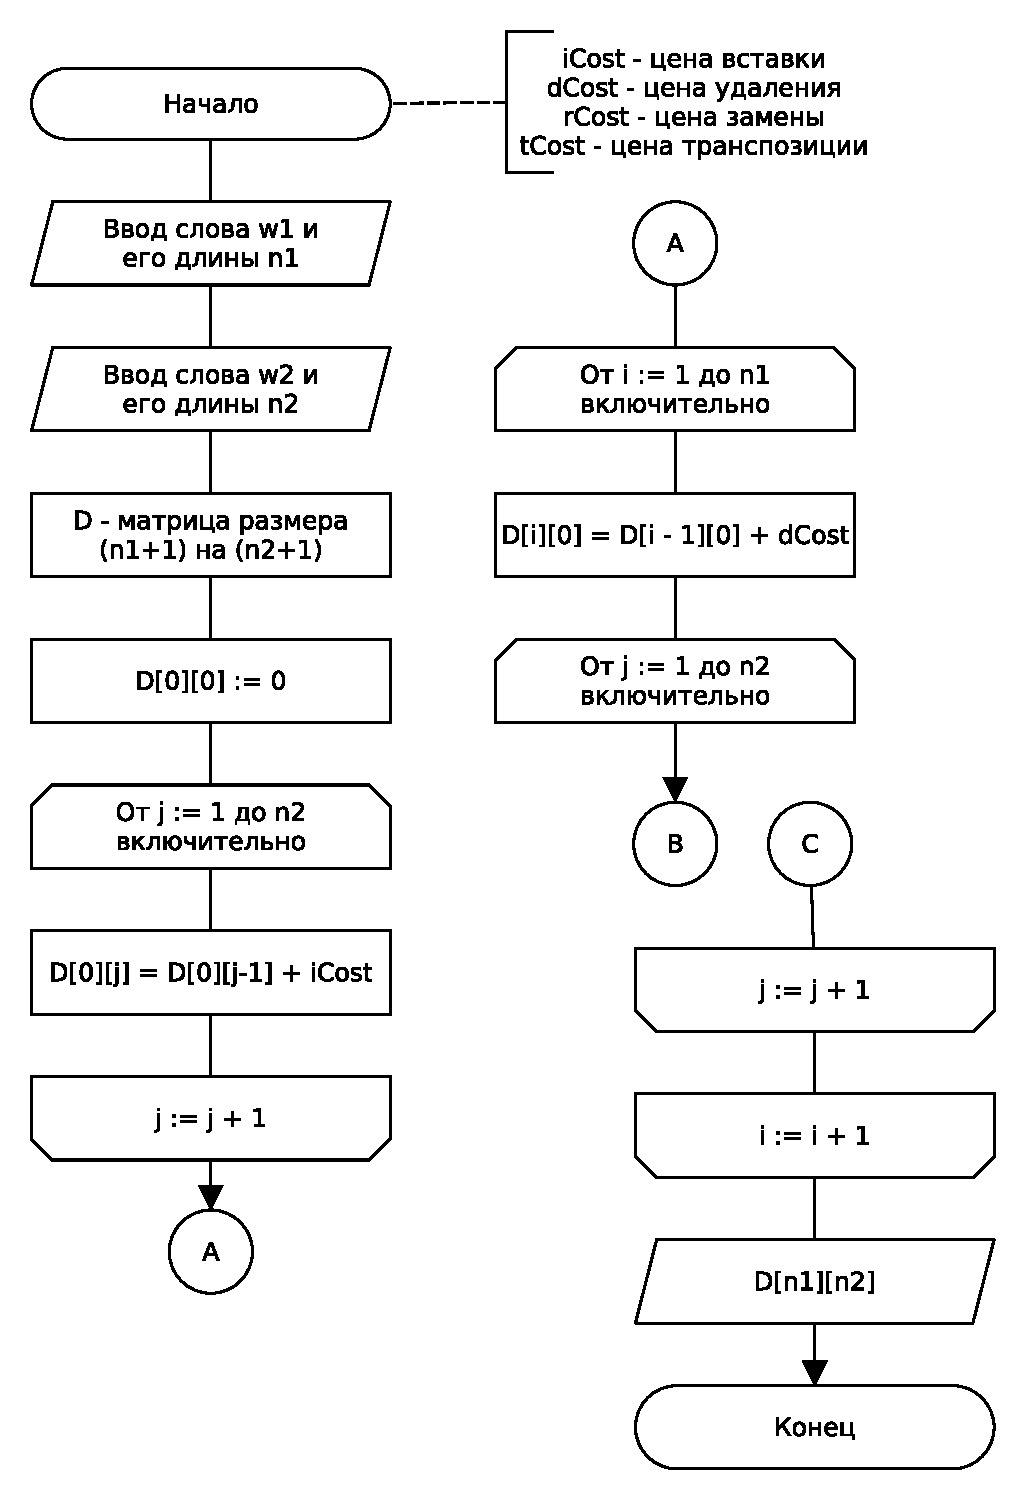
\includegraphics[scale=0.8]{pdf/damerau-levenshteain-part1.pdf}
    \caption{Матричный алгоритм Дамерау-Левенштейна, часть 1}
\end{figure}
\begin{figure}[H]
    \centering
    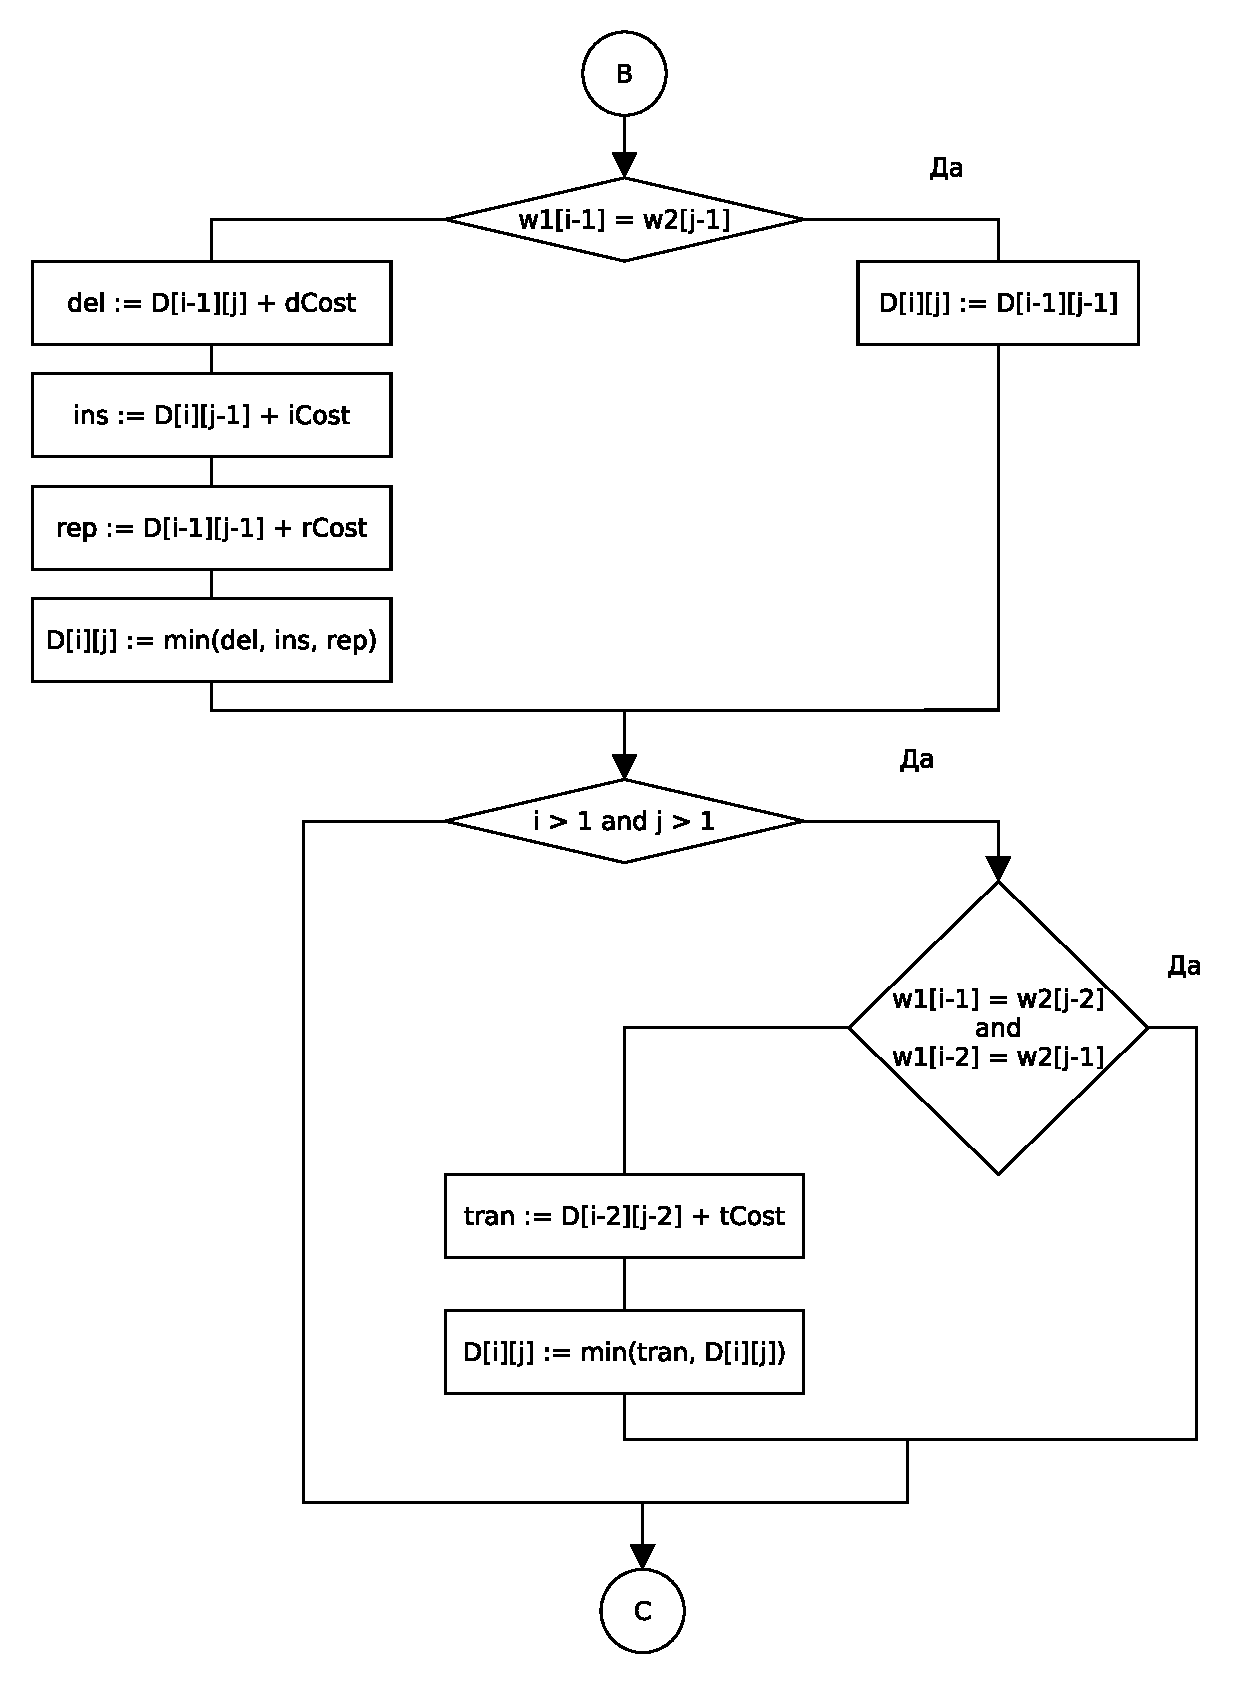
\includegraphics[scale=0.8]{pdf/damerau-levenshteain-part2.pdf}
    \caption{Матричный алгоритм Дамерау-Левенштейна, часть 2}
\end{figure}

\subsection{Рекурсивный алгоритм Дамерау-Левенштейна}


